
\documentclass[11pt,letterpaper ,oneside ,openright]{book}

\usepackage[pass]{geometry}

\usepackage{glossaries}
\usepackage{glossary-mcols}
\usepackage{yourStyleFile}

\usepackage{stackengine}
%\usepackage{pdflscape}
\usepackage{epigraph}
\setlength{\epigraphwidth}{0.9\textwidth}
\usepackage{chngcntr}
%\counterwithin{exx}{chapter}

%%% Stuff used for the title page %%%

% Include the textpos package
\usepackage[absolute,overlay]{textpos}

\definecolor{seeblau}{RGB}{0, 169, 224}
\setulcolor{seeblau}
\setul{0.1ex}{0.2ex}

\newcommand{\tinyspace}{\nobreak\hspace{.16667em}}



%\usepackage[left=2.5cm,right=2.5cm,top=2cm,bottom=2.5cm]{geometry}

\title{\bf Your title}

\author{Your name}
\date{University of Konstanz}





\begin{document}


%\maketitle

% -----------------------
% 1. Title page
% -----------------------

\newgeometry{hmarginratio=1:1,bottom=1cm}
\thispagestyle{empty}
\begin{center}
  \begin{sffamily}
    \begin{bfseries}
      \begin{LARGE}
	%\vspace*{8mm}
	% if \ul{} is used over multiple lines, centering is fucked up. Therefore: one \ul{} for every line
	\mbox{\ul{Your title}}\\% 
	\mbox{\ul{Line 2}}\\%
	\mbox{\ul{Line 3}}\\%
    %Adjust spaces between elements with vspace (may depend on length of title, etc.)
	\vspace{15mm}
      \end{LARGE}
      \begin{Large}
	\Large
    Master's thesis \\
	% Doctoral thesis for obtaining the\\[0.6\baselineskip]
	% academic degree\\[0.6\baselineskip]
	% Dr.{\tinyspace}rer.{\tinyspace}nat.\\
      \end{Large}
    \end{bfseries}
    \begin{mdseries}
      \begin{large}
	\vspace{12mm}
	submitted by \\[0.6\baselineskip]
	Your name\\
	\vspace{12mm}
	at the\\[\baselineskip]
	{
\includegraphics[width=0.5\textwidth]{upload/tex/figures/UniKonstanz-Logo-Optimum-sRGB.jpg}}\\
	\vspace{12mm}
	Faculty of Humanities\\[0.6\baselineskip]
	Department of Linguistics\\
      \end{large}
    \end{mdseries}
  \end{sffamily}

\end{center}

% Begin a text block with specified width at absolute position (x,y)
\begin{textblock*}{80mm}(20mm,235mm) % Adjust the coordinates (20mm, 270mm) as needed
  \large\mdseries\sffamily
  {
    \noindent
    1. Reviewer: Prof. name \\

    \noindent
    2. Reviewer: Prof. name
  }

      \null
  \vspace{4mm}
    \large\mdseries\sffamily
      \noindent
  Konstanz, 2020
\end{textblock*}

\restoregeometry


%Blank spaces for printing phd thesis
% \clearpage
% 	\afterpage{\blankpage}
% \clearpage
% 	\afterpage{\blankpage}
% \clearpage
% \afterpage{\blankpage}
% \clearpage
	

%\hfill{}
%\clearpage
%	\afterpage{\blankpage}
%\clearpage
%%	\afterpage{\blankpage}
%\clearpage

%Deep in the human unconscious is a pervasive need for a logical universe that makes sense. But the real universe is always one step beyond logic.
%-- from "The Sayings of Muad'Dib"
%by the Princess Irulan

% -----------------------
% Pre-amble: abstract, table of contents, glossary, etc.
% -----------------------
	
		\pagestyle{plain}
	% set Roman page numbers

	% acknowledgements
	\pagenumbering{roman}

	\section*{Abstract}

	\clearpage
	\section*{Zusammenfassung}


\clearpage
\afterpage{\blankpage}

	\clearpage
	\afterpage{\blankpage}
\clearpage
	\section*{Acknowledgements}


\clearpage

\glsaddall
\printnoidxglossary[type=main,style=mcolindex,nonumberlist]

% table of contents
\tableofcontents
\clearpage
\listoffigures
\clearpage
\listoftables
\clearpage
\afterpage{\blankpage}
\clearpage


\pagestyle{fancy}
\fancyhead{}
\fancyfoot[CO,CE]{\thepage}
	\fancyhead[RE]{\small \rightmark}
\fancyhead[LO]{\small \leftmark}
	\pagenumbering{arabic}
	% begin Arabic page numbers
	

\chapter{Introduction}
\label{chapter1}

This is the introduction. Here is a section.

\section{Your first section}

And this is a subsection.

\subsection{Your first subsection}

And here are some citations. First this \cite{kalouli2022negation}. (This is a citation in parenthesis \citealt{kalouli2022negation}). This is with a page number \citep[p. 5]{kalouli2022negation}. \citet{kalouli2022negation} says very smart things.

\section{Figure example}

Here is an example figure:

\begin{figure}
    \centering
    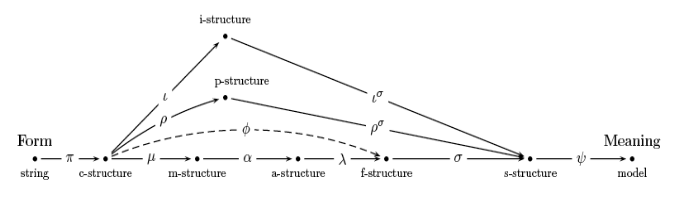
\includegraphics[scale=0.5]{upload/tex/figures/parallelprojection.png}
    \caption{This is the projection architecture}
    \label{fig-label1}
\end{figure}

Figure \ref{fig-label1} describes the projection architecture. 

\section{Linguistic exmaples}

You can refer to examples with \texttt{\\ref}. Like this \ref{ex:intro:ex1}.

\ex. \label{ex:intro:ex1} This is a simple linguistic example. 

\ex. Some text here 
\a. This is an example with subexamples
    \b. Second example


Here is an example with glossing.

\exg. The first line \\
    det first line \\
    \trans \textit{`The translation'}

\exg. The first line \\
    det {second first} line \\
    \trans \textit{`The translation'}

    This page explains linguistic examples: \url{https://ftp.tu-chemnitz.de/pub/tex/macros/latex/contrib/linguex/doc/linguex-doc.pdf}

    This sentence has a footnote.\footnote{This is a footnote.}

    \section{Tables}

    Go to \url{https://www.tablesgenerator.com/} to create tables:

    \begin{table}[]
    \centering
\begin{tabular}{l||ll}
a  & \multirow{3}{*}{b} & c  \\
1  &                    & 3  \\
ho &                    & ho
\end{tabular}
\caption{This is an example table}
\label{table:hohoho}
\end{table}

This is a reference to Table \ref{table:hohoho}

\section{Special symbols}

Use \url{https://detexify.kirelabs.org/classify.html} to find special symbols
	\chapter{Background}
\label{background}



	\chapter{chapter2 title}
\label{chapter2}


	\chapter{Figures}
\label{ch:figures}

% h means here: Place the figure in the text where the figure environment is written, if there is enough room left on the page
% t means top: Place it at the top of a page.
% b means bottom: Place it at the bottom of a page.
% p means page: Place it on a page containing only floats, such as figures and tables.

% ! allows to ignore certain parameters of LaTeX for float placement (think of it as forcing a parameter)

\begin{figure}[!h]  
    \centering
    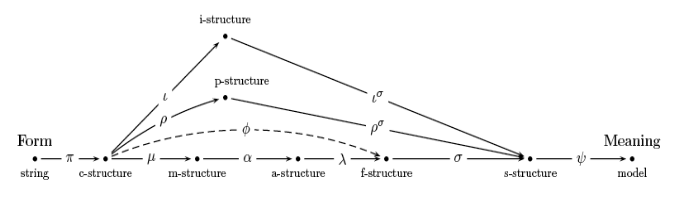
\includegraphics[scale=0.5]{upload/tex/figures/parallelprojection.png}
    \caption{This is the projection architecture}
    \label{fig-label1}
\end{figure}

\begin{figure}[!b]  
    \centering
    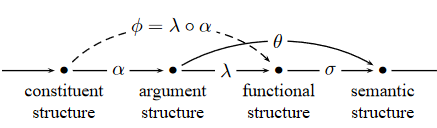
\includegraphics[width=.9\textwidth]{upload/tex/figures/mapping-functions.png}
    \caption{Mapping functions}
    \label{fig-label1}
\end{figure}

\begin{figure}[!t]  
    \centering
    
\includegraphics[height=1cm]{upload/tex/figures/UniKonstanz-Logo-Optimum-sRGB.jpg}
    \caption{Uni Konstanz Logo}
    \label{fig-label1}
\end{figure}
	\chapter{Linguistic structures}
\label{ch:chapter4}


\ex. \begin{minipage}[t]{.4\textwidth}
\textbf{Constituent structure:} \\
\Tree [.IP [.NP Jordan  ]  [.I$'$ [.VP [.V visited ] [.NP Alex ] ] ] ]
    \end{minipage}%
    \begin{minipage}[t]{.5\textwidth}
     \textbf{Semantics:} \\
       \begin{center}
         	\begin{prooftree}
		\AxiomC{$\lambda x. \lambda y.\text{visit}(y,x): g \multimap (h \multimap f)$}
		\AxiomC{$a : g$}
		%\RightLabel{$\multimap_{E}$}
		\BinaryInfC{$\lambda y.\text{visit}(y,a): h \multimap f$}
		    \AxiomC{$j : h$}	
\BinaryInfC{$\text{visit}(j,a): f$}
	\end{prooftree}
    \end{center}
    \end{minipage} \\%
    \hspace*{\fill}\\ 
    \begin{minipage}[t]{.4\textwidth}
    \textbf{Functional structure:} \\
    \hspace*{\fill}\\ 
    \begin{avm}
     \[ \avmspan{PRED `$<$Jordan, Alex$>$'} \\
        SUBJ & \[ PRED `Jordan' \] \\
        OBJ & \[ PRED `Alex' \] \\ 
        TENSE past \]
    \end{avm}
    \end{minipage}%
    \begin{minipage}[t]{.5\textwidth}
    \textbf{Discourse representation/model:}\\%
    \hspace*{\fill}\\
    \drs{e,x,y,t,n}{visit(e) \\ ag(e) = x \\ th(e) = y \\ x = Jordan  \\ y = Alex \\ e $\subseteq$ t \\ t $\prec$ n }
    \end{minipage}%


\section{Trees}

%Tree drawn with qtree syntax
\ex. \Tree [.IP [.NP Jordan ] [.I$'$ [.VP$_{[fin]}$ [.V seems ] [.CP [.C$'$  [.C to ] [.VP$_{[inf]}$ [.V like ] [.NP Alex ] ] ] ] ] ] ]

%Tikz-qtree version with additional options
\begin{figure}[!h]
\begin{center}
\begin{tikzpicture}
\Tree [.AP 
    [.A \edge[roof]; {tall +comp} ] 
    [.CP 
        [.C than ] 
        [.NP \edge[roof]; {the cat} ]
    ] 
]
\end{tikzpicture}
\end{center}
\caption{Often trees are best treated as figures}
\end{figure}

\ex. \begin{dependency}
\begin{deptext}
John \& kissed \& a \& girl \\
NNP/1 \& VBD/2 \& DET/3 \& NP/4 \\
% \& Tense=past \& \\
% \& VerbForm=fin \& \\
\end{deptext}
\depedge{2}{4}{obj}
\depedge{3}{4}{det}
\depedge{2}{1}{nsubj}
\deproot{2}{root}
\end{dependency}

\begin{footnotesize}
\begin{tikzpicture}
    \tikzset{every tree node/.style={align=center,anchor=north}}
\tikzset{grow'=up}
\tikzset{level 1+/.style={level distance=30pt}}
\tikzset{frontier/.style={distance from root=180pt}}
\Tree 
[.{FA}
                [.{FA} 
                    [.{} \node(14){$s_t \multimap f_t \multimap f_t$\\14}; ] 
                    [.{FA} 
                        [.{} \node(15){$s_e \multimap s_t$\\15}; ] 
                        [.{} \node(18){$s_e$\\18}; ] 
                    ] 
                ] 
    [.{FA}
                [.{FA} 
                    [.{} \node(16){$g_t \multimap f_t \multimap f_t$\\16}; ] 
                    [.{FA} 
                        [.{} \node(17){$g_e \multimap g_t$\\17}; ] 
                        [.{} \node(20){$g_e$\\20}; ] 
                    ] 
            ]
                [.{FA} 
    [.{FA} 
        [.{FA} 
                [.{} \node(13){$h_e \multimap s_e \multimap g_e \multimap f_t$\\13}; ]  
                  [.{} \node(12){$h_e$\\12}; ] 
            ]
             [.{} \node(19){$s_e$\\19}; ] 
            ]
            [.{} \node(21){$g_e$\\21}; ] 
            ]
        ] 
    ]
\end{tikzpicture}
\end{footnotesize}

\section{Fancy examples}

Projection architecture:

\begin{minipage}[t]{.3\textwidth}
\Tree [.{\tikznode{snor}{S}} [.{\tikznode{vpnor}{VP}} 
[.V {Joi-\textcircled{n}} ] 
[.{\tikznode{npnor}{NP}} kahvia ] ]  ]
\end{minipage}%
\begin{minipage}[t]{.5\textwidth}
\begin{avm}
{{\tikznode{fstrnor}{$f$}}}\[ \avmspan{PRED `drink$<$pro,coffee$>$'} \\
OBJ & {{\tikznode{fstrobjnor}{$h$}}}\[PRED `coffee' \\
NUM sg \\ PERS 3 \\ CASE partitive \] \\
SUBJ & {{\tikznode{fstrsubjnor}{$g$}}}\[PRED `pro' \\
NUM sg \\ PERS 1 \] \\
\avmspan{TENSE past}
\]
\end{avm}
\end{minipage}
\begin{tikzpicture}[overlay, remember picture]

    % Manual node placement (Corresponding to the left daughters of the tree)
    \node[overlay] at (-9.2,-3.05) (morphnor) {}; % Adjust coordinates as needed
    \node[overlay] at (-9.5,-2) (vnor) {}; % Adjust coordinates as needed

    % Arrow from c1 to c1s
\draw[->, bend right=10, looseness=1,-latex] 
    (snor) to [out=20, in=190] 
         (fstrnor.west);

\draw[->, bend right=10, looseness=1,-latex] 
    (vpnor) to [out=20, in=180] 
         (fstrnor.west);

\draw[->, bend right=10, looseness=1,-latex] 
    (vnor) to [out=30, in=165] 
         (fstrnor.west);

    \draw[->, bend right=5, looseness=0.9,-latex] 
        (npnor) to [out=330, in=220] 
             (fstrobjnor);

        \draw[->, bend right=5, looseness=0.9,-latex] 
        (morphnor) to [out=330, in=220] 
             (fstrsubjnor);    
\end{tikzpicture}\\
\strut \hfill{(based on \citealt{toivonen2023pronoun}: ex.~(6))} \\





\begin{figure}[!h]
\centering
\begin{tikzpicture}
   \tkzInit[xmax=6,ymax=4,xmin=0,ymin=0]%
   %\tkzGrid
   %\tkzAxeXY
    \tkzSetUpAxis[ticka=0pt, tickb=0pt]
   \tkzDrawX[label=t] \tkzDrawY[label=q]
  % \draw[->, thick] (0,2) -- (2,2) node[below]{post-state};
   \draw[->, thick] (0,1) -- node[below]{pre-state} ++(2,0);
   \draw[->, thick] (4,3) -- node[below]{post-state} ++(2,0);
      \draw[->, thick] (2,1) -- node[below]{\quad\quad\quad process} ++(2,2);
%   \draw[->, thick] (2,2) -- (4,6) node[above]{process};
%\draw[->, thick] (4,6) -- (6,6) node[below]{pre-state};

   % two points for drawing 2x+y=2
   %\tkzText[above](0,6.75){Desired Output}
  \end{tikzpicture}
  \caption{A diagram describing the temporal progression of an event}
  \label{ch4:fig:inner-asp-2d}
\end{figure}



\newpage
For typsetting movement-analyses, I manually position nodes, because somehow tikz struggles with nodes defined in the left branch of a tree. 

\ex. A rudimentary X$'$-analysis for minimalists \\
 \begin{minipage}[t]{.5\textwidth}
 $\approx$\textit{The chicken can start eating.} \\
 \Tree [.IP [.NP \edge[roof]; {the chicken$_1$} ] [.I$'$ [.I is ] [.VP [.AP ready ] [.CP [.{$t_1$} ] [.C$'$ [.C to ] [.VP eat ] ] ] ] ] ] 
\end{minipage}%
\begin{minipage}[t]{.5\textwidth}
 $\approx$\textit{The chicken is ready to be eaten.} \\
 \Tree [.IP [.NP \edge[roof]; {the chicken$_2$} ] [.I$'$ [.I is ] [.VP [.AP ready ] [.CP [.\textsc{pro} ] [.C$'$ [.C to ] [.VP [.V eat ] [.{\tikznode{readysyntrace2}{$t_2$}} ] ] ] ] ] ] ]
\end{minipage}
\begin{tikzpicture}[overlay, remember picture]
    % Manual node placement
    \node[overlay] at (7.7,5.5) (readysynp2) {}; % Adjust coordinates as needed
    \node[overlay] at (4.4,3.3) (readysyntrace1) {}; % Adjust coordinates as needed
        \node[overlay] at (1.3,5.5) (readysynp1) {}; % Adjust coordinates as needed
    % Arrow from c1 to c1s
    \draw[->, dashed, bend right=5, looseness=1] 
        (readysyntrace1) to [out=120, in=130] 
             (readysynp1); 
    % Arrow from c2 to c2s
    \draw[->, dashed, bend right=5, looseness=1.5] 
        (readysyntrace2) to [out=120, in=130]
          (readysynp2);
\end{tikzpicture}
  




	\chapter{chapter 5 title}
\label{chapter5}


	 %chapters
	 
	 \printbibliography

\end{document}